\chapter{Survey of Past Verification and Validation Work}

\label{Survey_Chapter}

CFAST has been subjected to extensive validation studies by NIST and others. This chapter provides a review of select CFAST validation efforts by NIST and others to better understand the quality of the predictions by the model. Some of the work has been  performed at NIST, some by its grantees and some by engineering firms using the model.  Because each organization has its  own reasons for  validating the model, the  referenced papers and reports do not follow any particular guidelines. Some of the works only provide  a qualitative assessment  of the model,  concluding that the  model  agreement with  a  particular  experiment  is ``good''  or ``reasonable.'' Sometimes, the conclusion is that the model works well in certain cases, not as well in others. These studies are included in the survey because the references  are useful to other model users who may have a similar application  and are interested in qualitative assessment. It is important to note  that some of the papers point out flaws in early releases of CFAST that have been corrected or improved in more recent  releases.

\section{Model Sensitivity}

A sensitivity analysis considers the extent to which uncertainty in model inputs influences model output.  For a sensitivity analysis, this uncertainty includes not only that inherent in the input of data for specific scenarios by the model user, but also uncertainty in empirical data or numerical parameters in the model such as the time step size used by the model to obtain a solution. Iman and Helton~\cite{Iman:1988} studied the sensitivity of complex computer models developed to simulate the risk of severe nuclear accidents which may include fire and other risks. Consistent with the work of Iman and Helton, ASTM E1355~\cite{ASTM:E1355} provides overall guidance on typical areas of evaluation of the sensitivity of deterministic fire models.  These areas may involve one or more of the following techniques: finite difference or direct analysis methods that provide an explicit solution of the sensitivity equations associated with the governing equations of the model, factorial design or Latin hypercube sampling studies that investigate the effect of varying the input parameters and consequential interactions between parameters that may be deemed important, and global or response surface methods that investigate the overall behavior of model outputs for a desired range of inputs.

This section provides a review of the sensitivity studies that have been conducted using CFAST with an emphasis on uncertainty in the input. Other sensitivity investigations of CFAST are also available \cite{Peacock:1988a, Beard:1992, Notarianni:2000}.

Khoudja~\cite{Khoudja:1988} has studied the sensitivity of an early version of FAST (the predecessor of CFAST) with a fractional factorial design involving two levels of 16 different input parameters. The statistical design, taken from the texts by Box and Hunter~\cite{Box:1978} and Daniel~\cite{Daniel:1976} reduced the necessary model runs from more than 65,000 to 256 by studying the interactions of input parameters simultaneously. The choice of values for each input parameter represented a range for each parameter. The analysis of the FAST model showed sensitivity to heat loss to the compartment walls and to the number of compartments in the simulation.

Walker~\cite{Walker:1997} discussed the uncertainties in components of zone models and showed how uncertainty within user-supplied data affects the results of calculations using CFAST as an example. The study systematically varied inputs related to the fire (heat release rate, heat of combustion, mass loss rate, radiative fraction, and species yields) and compartment geometry (vent size and ceiling height). Heat release rate and ceiling height are seen to be the dominant input variables in the simulations.

Peacock et al.~\cite{Peacock:1988a} studied the sensitivity of CFAST for a range of input parameters. They used simple factorial designs for model inputs deemed important to investigate local behavior of important model outputs along with response surface methods to evaluate overall model behavior.


\section{Comparisons of CFAST with Full-Scale Experiments}

Several studies have been conducted specifically to validate the use of CFAST in building performance design. Dembsey~\cite{Valid:Dempsey} used CFAST version 3.1 to predict the ceiling jet temperatures, surface heat fluxes and heat transfer coefficients for twenty compartment fire experiments in a compartment that is similar in size, geometry, and construction to the standard fire test compartment specified in the Uniform Building Code~\cite{UBC}. Results from 330 kW, 630 kW, and 980 kW fires were used. In general, CFAST made predictions which were higher than the experimental results. In these cases, the temperature prediction was typically 20~\% to 30~\% higher than measured values. Much of this can be attributed to not knowing the species production (soot) and relative absorption of radiation by the gas layers which highlights the importance of scenario specification. This is the most common cause of  ``over prediction'' of temperature by CFAST. A secondary source of discrepancy is correcting for thermal radiation of thermocouple beads. The authors provide for this correction, but the corrections cited are not as large as has been reported in other fire experiments~\cite{Valid:Pitts}.

He et al.~\cite{Valid:He} describe a series of full-scale fire experiments that were designed to investigate the validity of two zone models including CFAST version 3.1. The experiments, involving steady state burning rates and a number of ventilation conditions, were conducted in a four-story building. Temperature, pressure, flow velocity, smoke density and species concentrations were measured in various parts of the building. The stack effect and its influence on temperature distribution in a stair shaft were observed. Comparisons were then made between the experimental results and the model predictions. Early in the fire there is a few percent difference between the predictions and measurements; beyond 10 min, there are significant variations. Both the experiment and the model are internally consistent; that is, higher flow leads to a higher interface height (figure 13 in the paper). Once again, the difference is about 25~\%. The authors discuss the effect of fuel composition and correction for radiation to/from thermocouple beads but did not draw firm conclusions based on their measurements of fuel products.

A series of experimental results for flaming fires, obtained using realistic fires in a prototype apartment building were performed by Luo et al.~\cite{Valid:Luo}. Fuel configurations in the fire test included a horizontal plain polyurethane slab, mock-up chair (polyurethane slabs plus a cotton linen cover), and a commercial chair. CFAST version 3.1 typically over-predicted upper layer temperatures by 10 \% to 50 \% depending on the test conditions and measurement location in that test. The predicted and experimental time dependent upper layer temperatures were similar in shape. The time to obtain peak upper layer temperatures was typically predicted to within 15 \% of the experimental measurements. The authors concluded that CFAST was conservative in terms of life safety calculations.

Poole et al.~\cite{Valid:Poole} reported the results of a cooperative project between the Kitchener, Ontario, Fire Department and the University of Waterloo aimed at developing design criteria for the construction of a fire fighter training facility. One particular criterion is that realistic training with respect to temperature, heat release and stratification be provided in such a facility. The purpose of this paper was to compare existing analytical heat release and upper and lower gas temperature rise correlations and models with data from actual structures which were instrumented and burned in collaboration with the Kitchener Fire Department. According to the authors, the CFAST model was used ``successfully'' to predict these conditions and will be used in future design of such facilities.

A report by Bailey et al.~\cite{Valid:Bailey_Shadwell} compares predictions by CFAST version 3.1 to data from real scale fire tests conducted onboard ex-USS SHADWELL, a decommissioned naval vessel. The phenomenon of particular interest in this validation series was the conduction of heat in the vertical direction through compartment ceilings and floors. As part of this work, Bailey et al.~\cite{Valid:Bailey_Vertical_Heat} compared CFAST temperature predictions on the unexposed walls of large metal boxes, driven by steady state fires. This tested the model's prediction of radiation and conduction in both the vertical and horizontal directions. The model and experiment compared well within measurement error bounds of each. The comparison was particularly good for measurements in the fire compartment as well as for the compartment and deck directly above it, with predictions typically agreeing with experiments within measurement uncertainty. The model under-predicted the temperatures of the compartments and decks not directly adjacent to the fire compartment early in the tests.

Deal \cite{Valid:Deal} reviewed four computer fire models (CCFM \cite{Models:CCFM}, FIRST \cite{Models:FIRST}, FPETOOL \cite{Models:FPETool} and FAST \cite{Models:FAST} version 18.5 (the immediate predecessor to CFAST)) to ascertain the relative performance of the models in simulating fire experiments in a small room (about 12 m$^3$ in volume) in which the vent and fuel effects were varied. Peak fire size in the experiments ranged up to 800~kW. According to the author, all the models simulated the experimental conditions including temperature, species generation, and vent flows ``quite satisfactorily.''

Matsuyama conducted a series of full-scale experiments~\cite{Matsuyama:2000} using t$^2$ fires \footnote{For a range of fires, the fire growth can be represented with a power law relation of the form $\dq = \alpha \; t^2$ where $\dq$ is the heat
release rate of the fire, $\alpha$ is the fire intensity coefficient, and $t$ is time}. Fire room and corridor smoke filling processes were measured. The size of the corridors and arrangements of smoke curtains were varied in several patterns. Comparisons were then made between the experimental results and those predicted by CFAST. The author concludes that while the model does a ``good job'' of predicting experimental results, there are systematic differences which could be reduced with some revision to zone model formulation to include the impact of smoke curtains.

\subsection{Fire Plumes}

Davis compared predictions by CFAST version 5 (and other models) for high ceiling spaces~\cite{Valid:Davis_Plumes}. In this paper, the predictive capability of two algorithms designed to calculate plume centerline temperature and maximum ceiling jet temperature in the presence of a hot upper layer were compared to measurements from experiments and to predictions using the CFAST ceiling jet algorithm. The experiments included ceiling heights of 0.58~m to 22~m and heat release rates of 0.62~kW to 33~MW. When compared to the experimental results, the ceiling jet algorithm tended to over-predict the upper layer temperature by 20~\%. With proper adjustment for radiation effects in the thermocouple measurements, some of this difference disappears. The effect of entrainment of the upper layer gases was identified for improvement.

\subsection{Multiple Compartments}
\label{secMultipleCompartments}

Jones and Peacock \cite{Valid:Jones} presented a limited set of comparisons between the FAST model (version 18.5) and a multi-room fire test. The experiment involved a constant fire of about 100 kW in a three-compartment configuration of about 100 m$^3$. They observed that the model predicted an upper layer temperature that was too high by about 20 \% with satisfactory prediction of the layer interface position. These observations were made before the work of Pitts et al. \cite{Valid:Pitts} showed that the thermocouple measurements need to be corrected for radiation effects. Convective heating and plume entrainment were seen to limit the accuracy of the predictions. A comparison of predicted and measured pressures in the rooms showed accuracy within 20 \%. Since pressure is the driving force for flow between compartments, this agreement was seen as important.

Levine and Nelson \cite{Valid:Levine} used a combination of full-scale fire testing and modeling to simulate a fire in a residence. The 1987 fire in a first-floor kitchen resulted in the deaths of three persons in an upstairs bedroom, one with a reported blood carboxyhemoglobin content of 91 \%. Considerable physical evidence remained. The fire was successfully simulated at full scale in a fully-instrumented seven-room two-story test structure. The data collected during the test have been used to test the predictive abilities of two multiroom computer fire models: FAST and HARVARD VI. A coherent ceiling layer flow occurred during the full-scale test and quickly carried high concentrations of carbon monoxide to remote compartments. Such flow is not directly accounted for in either computer code. However, both codes predicted the carbon monoxide buildup in the room most remote from the fire. Prediction of the pre-flashover temperature rise was also `good' according to the authors. Prediction of temperatures after flashover that occurred in the room of fire origin was seen as `less good.' Other predictions of conditions throughout the seven test rooms varied from `good approximations' to `significant deviations' from test data. Some of these deviations are believed to be due to combustion chemistry in the hot upper layer not considered in detail in either of the two models.

\subsection{Large Compartments}

Duong \cite{Valid:Duong} studied the predictions of several computer fire models (CCFM, FAST, FIRST, and BRI \cite{Models:BRI}), comparing the models with one another and with large fires (4 MW to 36 MW) in an aircraft hanger (60 000 m$^3$). For the 4 MW fire size, he concluded that all the models are `reasonably accurate.' At 36 MW, however, `none of the models did well.' Limitations of the heat conduction and plume entrainment algorithms were thought to account for some of the inaccuracies.

\subsection{Mechanical Ventilation}

There have been two papers which have looked at the effectiveness of the mechanical ventilation system. The first considered a fire chamber of length 4.0 m, width 3.0 m and height 2.8 m with adjustable ventilation rates \cite{Chow:1995a}. Burning tests were carried out with wood cribs and methanol to study the preflashover stage of a compartmental fire and the effect of ventilation. The mass loss rate of fuel, temperature distribution of the compartment and the air intake rate were measured. The heat release rates of the fuel were calculated and the smoke temperature was used as a validation parameter. A scoring system was proposed to compare the results predicted by the three models. According to the author, CFAST does `particularly well,' though there are some differences which can be attributed to the zone model approach.

A second series of experiments by Luo \cite{Luo:1997} indicate that the CFAST model (version 3.1) generally over-predicts the upper layer temperature in the burn room because the two-zone assumption is likely to break down in the burn room. It was found that the room-averaged temperatures obtained from CFAST were in `good overall agreement' with the experimental results. The discrepancies can be attributed to the correction needed for thermocouple measurements. The CO concentration,however, was inconsistent. CFAST tended to overestimate CO concentration when the air handling system was in operation. This was seen due to inconsistencies in what is measured (point measurements) and predicted (global measurements).

\subsection{Sprinkler Activation}

A suppression algorithm \cite{Madrzykowski:1992} was incorporated into CFAST. Chow \cite{Chow:1996a} evaluated the predictive capability for a sprinkler installed in an atrium roof. There were three main points being considered: the possibility of activating the sprinkler, thermal response, and water requirement. The zone model CFAST was used to analyze the possibility of activation of a sprinkler head. Results derived from CFAST were seen to be `accurate, that is, providing good agreement with experimental measurements.'

\subsection{Flashover}

Flashover is a term describing the transition of a relatively localized interior fire to one engulfing the entire compartment. It is of interest to the fire service because of the danger to fire fighters and to building designers because of life safety and the attendant impact on occupants. Several papers have looked at the capability of CFAST to predict the conditions under which flashover can occur.

Chow \cite{Valid:Chow_Flashover} concluded that FAST correctly predicted the onset of flashover if the appropriate criteria were used. The criteria were gas temperature near the ceiling, heat flux at the floor level and flames coming out of the openings. This analysis was based on a series of compartment fires.

A paper by Luo et al. \cite{Valid:Luo_Flashover} presents a comparison of the results from CFAST version 3 against a comprehensive set of data obtained from one flashover fire experiment. The experimental results were obtained from a full-scale prototype apartment building under flashover conditions. Three polyurethane mattresses were used as fuel. It was found that the predicted temperatures from the CFAST fire model agreed well with the experimental results in most areas, once radiation corrections are applied to the thermocouple data.

Collier \cite{Valid:Collier} makes an attempt to quantify the fire hazards associated with a typical New Zealand dwelling with a series of experiments. These tests, done in a three-bedroom dwelling, included both non-flashover and flashover fires. The predictions by CFAST version 2 were seen by the author as consistent with the experiments within the uncertainty of each.

Post-flashover fires in shipboard spaces have a pronounced effects on adjacent spaces due to highly conductive boundaries. CFAST (version 3.1) predictions for the gas temperature and the cold wall temperature were compared with shipboard fires \cite{Valid:White}. The comparisons between the model and experimental data show `conservative predictions' according to the authors. The authors attribute this to an overestimation of the average hot wall temperature and an underestimation of external convective losses due to wind effects.

Finally, a comparison of CFAST with a number of simple correlations was used by Peacock and Babrauskas \cite{Valid:Peacock_Flashover_1,Valid:Peacock_Flashover_2} to simulate a range of geometries and fire conditions to predict the development of the fire up to the point of flashover. The simulations represent a range of compartment sizes and ceiling heights. Both the correlations and CFAST predictions were seen to provide a lower bound to observed occurrence of flashover. For very small or very large compartment openings, the differences between the correlations, experimental data, and CFAST predictions was more pronounced.

The important test of all these prediction methods is in the comparison of the predictions with actual fire observations. Figure \ref{figValidFlashover} (reference \cite{Valid:Peacock_Flashover_2}) presents estimates of the energy required to achieve flashover for a range of room and vent sizes. This figure is an extension of the earlier work of Babrauskas  \cite{Valid:Babrauskas_Flashover} and includes additional experimental measurements from a variety of sources, most notably the work of Deal and Beyler \cite{Valid:DealandBeyler}. For a number of the experimental observations, values are included that were not explicitly identified as being a minimum value at flashover. In addition, figure \ref{figValidFlashover} includes predictions from the CFAST model (version 5).

\begin{figure}
\begin{center}
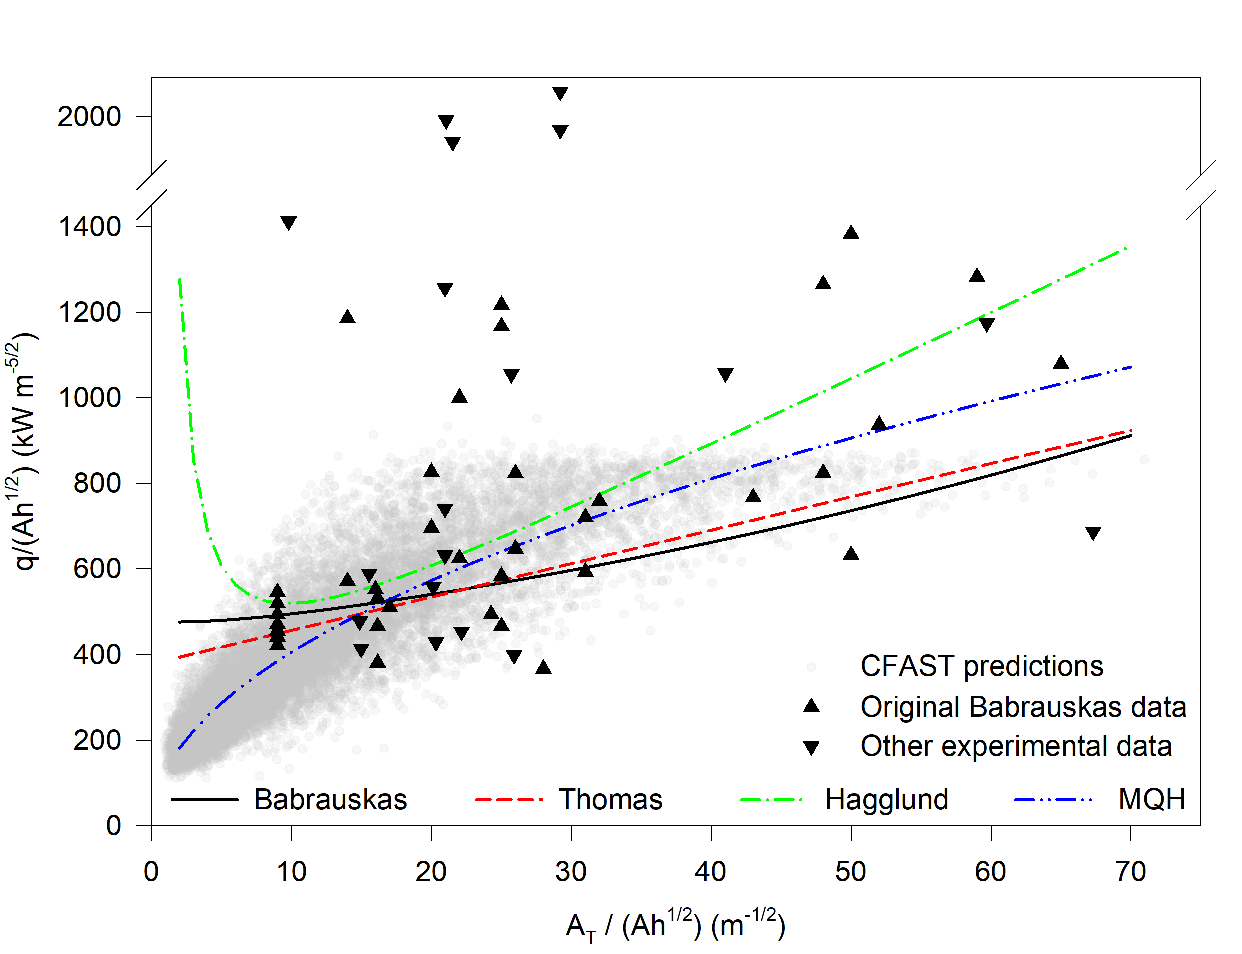
\includegraphics[width=5.0000in]{FIGURES/flashover.pdf}\\
\end{center}
\caption{Comparison of correlations, CFAST predictions, and experimental data for the prediction of flashover in a compartment fire.}
 \label{figValidFlashover}
\end{figure}

As with some of the experimental data defining flashover as an upper layer temperature reaching 600 $^{\circ}$C, many experimental measures were reported as peak values rather than minimum values necessary to achieve flashover. Thus, ideally all the predictions should provide a lower bound for the experimental data. Indeed, this is consistent with the graph -- the vast majority of the experimental observations lie above the correlations and model predictions. For a considerable range in the ratio \asqh, the correlations of Babrauskas \cite{Valid:Babrauskas_Flashover} Thomas \cite{Thomas:1981fk}, and the MQH correlation of McCaffrey et al. \cite{McCaffrey:1981uq} provide similar estimates of the minimum energy required to produce flashover. The estimates of H\"{a}gglund \cite{Hagglund:1980} yields somewhat higher estimates for values of \asqh  \, greater than 20 m$^{-1/2}$.

The results from the CFAST model for this single compartment scenario provide similar results to the experiments and the correlations for most of the range of \asqh. For small values of \asqh, the CFAST values rise somewhat above the values from the correlations. These small values of \asqh \, result from either very small compartments (small $A_T$) or very large openings (large \asqh), both of which stretch the limits of the assumptions inherent in the model. For very small compartments, radiation from the fire to the compartment surfaces becomes more important, enhancing the conductive heat losses through the walls. However, the basic two-zone assumption may break down as the room becomes very small. For very large openings, the calculation of vent flow via an orifice flow coefficient approach is likely inaccurate. Indeed, for such openings, this limitation has been observed experimentally \cite{Valid:Babrauskas_Flashover}. The estimates are close to the range of uncertainty shown by the correlations which also diverge at very small values of \asqh.

Perhaps most significant in these comparisons is that all the simple correlations provide estimates similar to the CFAST model and all the models are consistent with a wide range of experimental data. For this simple scenario, little is gained with the use of the more complex models. For more complicated scenarios, the comparison may not be as simple.

\section{Comparisons of CFAST with Actual Fires}

There are numerous cases of CFAST being used to adjudicate legal disputes. Since these are discussed in courts of law, there is a great deal of scrutiny of the modeling, assumptions, and results. Most of these simulations and comparisons are not available in the public literature. A few of the cases which are available are discussed below. The metric for how well the model performed is its ability to reproduce the time-line as observed by witnesses and the death of occupants or the destruction of property as was used in evidence in legal proceedings.

As mentioned in section \ref{secMultipleCompartments}, Levine and Nelson describe the use of FAST for understanding the deaths of two adults in a residence in Sharon, Pennsylvania in 1987 \cite{Valid:Levine}. The paper compared the evidence of the actual fire, a full scale mockup done at NIST and the results from FAST (version 18) \cite{Jones:1985} and Harvard VI \cite{Rockett:1985}. The most notable shortcoming of the models was the lower than actual temperatures in the bedrooms, caused by loss of heat through the fire barriers. This led to the improvement in CFAST in the mid-90s to couple compartments together so that both horizontal and vertical heat transfer can occur to adjacent compartments.

Bukowski used CFAST version 3.1 to analyze a fire in New York City \cite{Bukowski:1996} in 1994 which resulted in the death of three fire fighters. The CFAST model was able to reproduce the observed conditions and supported the theory as to how the fire began and the cause of death of the three fire fighters.

Chow describes the use and comparison of CFAST simulations with a 1996 high rise building fire in Hong Kong \cite{Chow:1996}. CFAST simulations were performed to help understand the probable fire environment under different conditions. Three simulations were performed to study the consequences of a fire starting in the lift shaft. Smoke flow in the simulations qualitatively matched those observed during the incident.

In the early morning hours of March 25,1990 a tragic fire took the lives of 87 persons at a neighborhood club in the Bronx, New York \cite{Bukowski:1992}. The New York City Fire Department requested the assistance of the NIST Center for Fire Research (CFR) in understanding the factors which contributed to this high death toll and to develop a strategy that might reduce the risk of a similar occurrence in the many similar clubs operating in the city. The simulation showed the potential for development of untenable conditions within the club and particularly in the single exit stairway.


\section{Comparisons of CFAST for Special Applications}

There are several sets of comparisons used in the development of the model or specific applications beyond those discussed more generally above.

\subsection{Nuclear Facilities}

Floyd validated CFAST version 3.1 by comparing the modeling results with measurements from fire tests at the Heiss-Dampf Reaktor (HDR) facility \cite{Floyd:2002}. The structure was originally the containment building for a nuclear power reactor in Germany. The cylindrical structure was 20 m in diameter and 50 m in height topped by a hemispherical dome 10 m in radius. The building was divided into eight levels. The total volume of the building was approximately 11 000 m$^3$. From 1984 to
1991, four fire test series were performed within the HDR facility. The T51 test series consisted of 11 propane gas tests and three wood crib tests. To avoid permanent damage to the test facility, a special set of test rooms were constructed, consisting of a fire room with a narrow door, a long corridor wrapping around the reactor vessel shield wall, and a curtained area centered beneath a maintenance hatch. The fire room walls were lined with fire brick. The doorway and corridor walls had the same construction as the test chamber. Six gas burners were mounted in the fire room. The fuel source was propane gas mixed with 10 \% air fed at a constant rate to one of the six burners.

In general, the comparison between CFAST and the HDR results was seen as `good' by the author, with two exceptions. The first is the over estimate of the temperature of the upper layer, typically within about 15 \% of the experimental measurements. This is common and generally results from using too low a value for the production of soot, water (hydrogen) and carbon monoxide. The other exception consists of predictions in spaces where the zone model concept breaks down, for example in the stairways between levels. In this case, CFAST has to treat the space either in the filling mode (two layer approximation) or as a fully mixed zone (using the SHAFT option). Neither is quite correct, and in order to understand the condition in such spaces in detail (beyond the transfer of mass and energy), a more detailed computational fluid dynamics model must be used, for example,  the Fire Dynamics Simulator (FDS) \cite{FDS_Tech_Guide_5}.

The U.S. Nuclear Regulatory Commission (NRC) performed an extensive verification and validation of several fire models commonly used in nuclear power plant applications \cite{NRCNUREG1824}.  These models included simple spreadsheet calculations, zone models (including CFAST), and CFD models. The results of this study are presented in the form of relative differences between fire model predictions and experimental data for fire modeling attributes such as temperature or heat flux that are important to NPP fire modeling applications.  These relative differences are affected by the capabilities of the models, the availability of accurate applicable experimental data, and the experimental uncertainty of these data. Evaluation of the two-zone models showed that the models simulated the experimental results within experimental uncertainty  for many of the parameters of interest. The reason for this may be that the relatively simple experimental configurations selected for this study conform well to the simple two-layer assumption that is the basis of these models.

While the relative differences sometimes show agreement for many parameters, they also show both under-prediction and over-prediction in some circumstances, most notably when conditions vary within a compartment or detailed local conditions are important to accurate prediction (for example, plume temperature or heat flux near to the fire source). The results and comparisons included the the NRC study are included in this report for the current version of CFAST.

\subsection{Small Compartments}

As an implementation of the zone model concept, CFAST is applicable to a wide range of scenarios. One end of this spectrum are small compartments, one to two meters on a side. Several research efforts have looked at small scale validation. There are three papers by Chow \cite{Lui:2003,Chow:1995,Chow:1992} which examine this issue. The first is the use of an electric heater with adjustable thermal power output was to verify temperature predictions by CFAST version 3.1. The second was closed chamber fires studied by burning four types of organic liquids, namely ethanol, N-heptane, and kerosene. The burning behavior of the liquids was observed, and the hot gas temperature measured. These behaviors along with the transient variations of the temperature were then compared with those predicted by the CFAST model. Finally, in another series of experiments, three zone models, one of which was CFAST, were evaluated experimentally using a small fire chamber. Once again, liquid fires were chosen for having better control on the mass loss rate. The results on the development of smoke layer and the hot gas temperature predicted by the three models were compared with those measured experimentally. According to Chow, `fairly good agreement' was found if the input parameters were carefully chosen.

\subsection{Railway and Vehicle Tunnels}

Altinakar et al. \cite{Altinakar:1997} used a \emph{modified version} of CFAST for predicting fire development and smoke propagation in vehicle or railroad tunnels. The two major modifications made to the model dealt with mixing between the upper and lower layers and friction losses along the tunnel. The model was tested by simulating several full-scale tests carried out at memorial Tunnel Ventilation Test Program in West Virginia, and the Offeneg Tunnel in Switzerland. His article compares simulated values of temperature, opacity and similar sensible quantities with measured values and discusses the limits of the applicability of zone models for simulating fire and smoke propagation in vehicle and railroad tunnels.

Peacock et al. \cite{Peacock:2004} compared times to untenable conditions determined from tests in a passenger rail car with those predicted by CFAST for the same car geometry and fire scenarios. For a range of fire sizes and growth rates, they found agreement that averaged approximately 13~\%.

\subsection{Non-Uniform Compartments}

In January 1996, the U.S. Navy began testing how the CFAST model would perform when tasked with predicting shipboard fires. These conditions include mass transport through vertical vents (representing hatches and scuttles), energy transport via conduction through decks, improvement to the radiation transport sub-model, and geometry peculiar to combat ships. The purpose of this study was to identify CFAST limitations and develop methods for circumnavigating these problems \cite{Hoover:2001}. A retired ship representing the forward half of a {USS} Los Angeles class submarine was used during this test series. Compartments in combat ships are not square in floor area, nor do they have parallel sides.

Application of CFAST to these scenarios required a direct integration of compartment cross-sectional area as a function of height to correctly interpret the layer interface position and provide correct predictions for flow through doors and windows (vertical vents). This required user specification of the area as a function of height to provide a description for the model to use.
